\documentclass[FinalReport.tex]{subfiles}
\begin{document}

\section*{\textsc{\Large Results}}

An initial way to view the performance of the Traces with specific Configurations is to look at the execution times for those Configurations.  Fig.~\ref{fig:executiontimes} shows each Trace and its execution time for each Configuration in relation to all the other traces.
\begin{figure}[H]
\centering
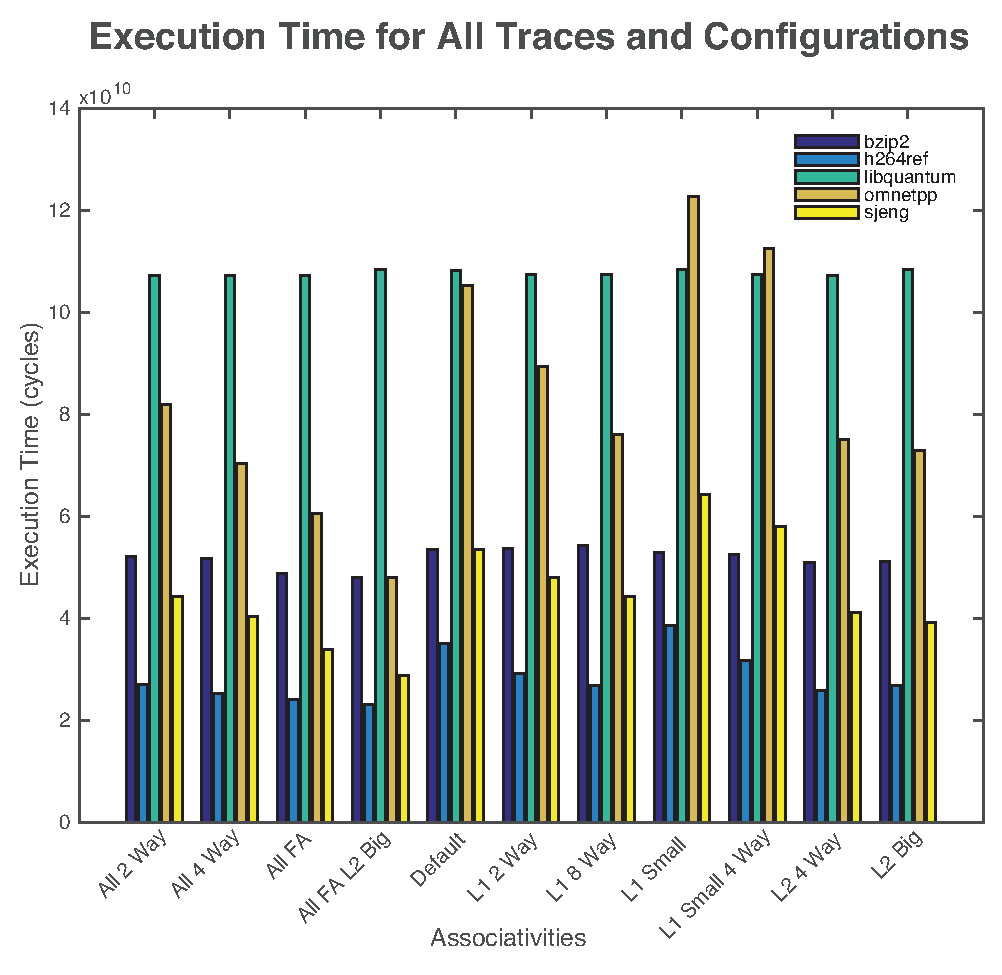
\includegraphics[scale = 0.75]{bargraph1.eps}
\caption{Execution times of all Traces with correspondence to all Configurations\label{fig:executiontimes}}
\end{figure}
The execution time for some traces varies very little with changes in cache configuration while other traces are largely effected by the cache configuration.  As seen in Fig.~\ref{fig:executiontimes}, {libquantum} has a very steady execution time which does not seem to depend on cache configuration.  A trace like {omnetpp} however, is very dependent on the cache configuration.  The execution times range from 40 billion cycles to 120 billion cycles. 

Another way to compare the performance of each trace is to look at the Cycles per Instruction (CPI).  This is plotted in Fig.~\ref{fig:CPI}.
\begin{figure}[H]
\centering
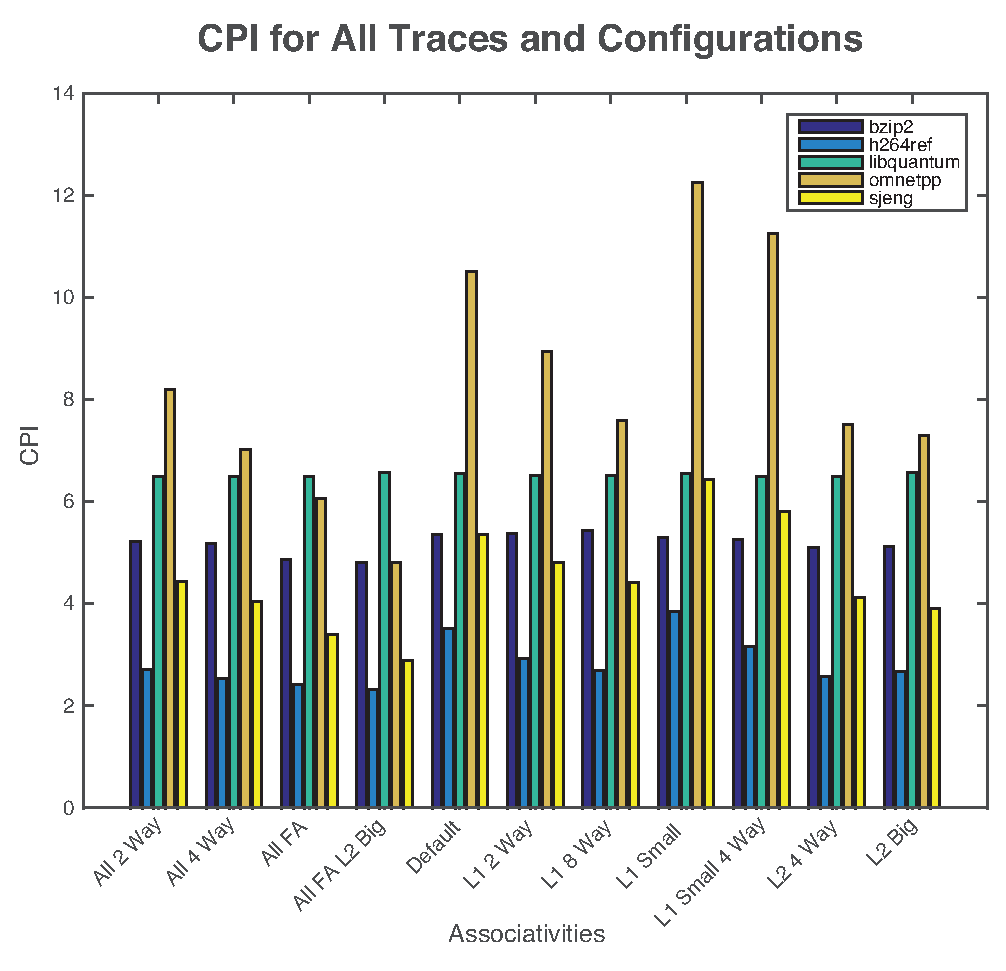
\includegraphics[scale = 0.75]{CPITimes.eps}
\caption{CPI of all Traces with correspondence to all Configurations\label{fig:CPI}}
\end{figure}
Similar to the execution times in Fig.~\ref{fig:executiontimes}, Fig.~\ref{fig:CPI} shows that the configuration of the cache can dramatically effect the CPI. 
\begin{center}
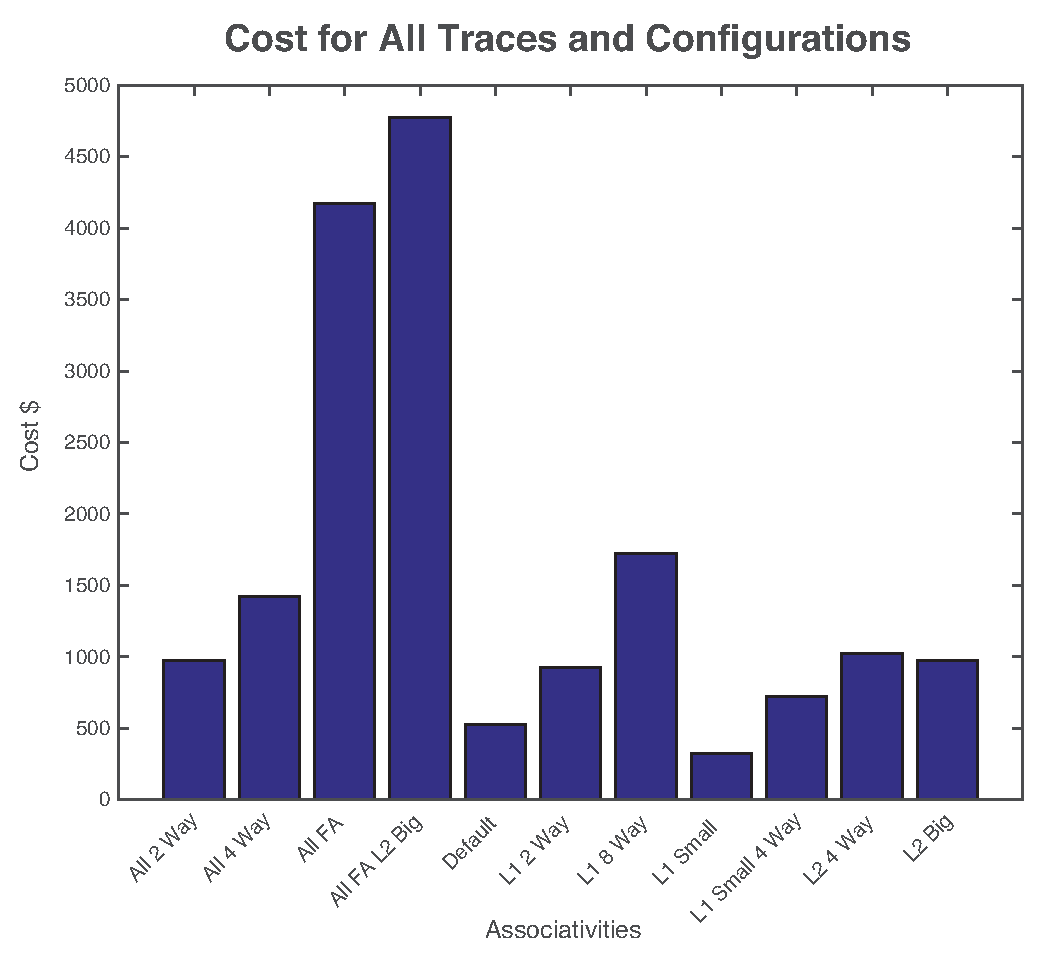
\includegraphics[scale = 0.75]{costVsConfig.eps}
\end{center}

\begin{center}
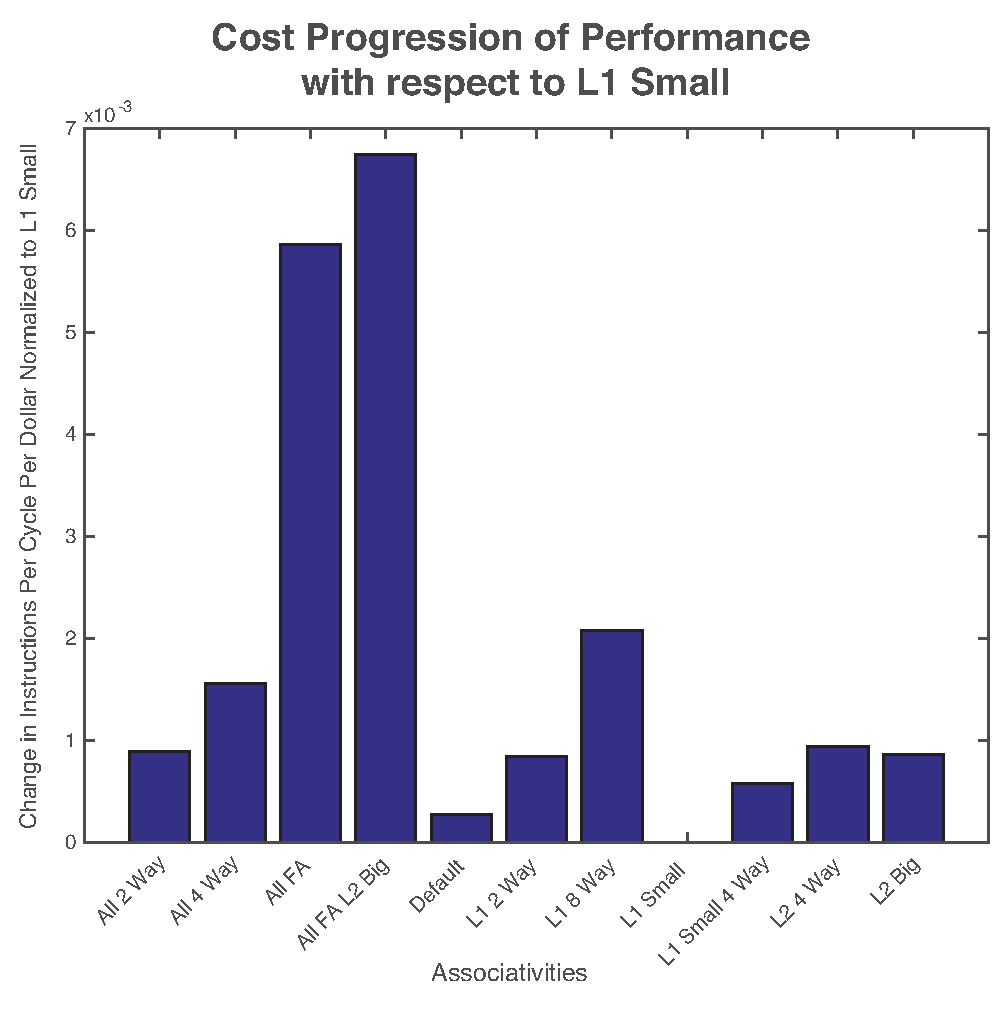
\includegraphics[scale = 0.75]{IPCperDollarDiff_wrtL1Small.eps}
\end{center}


\begin{center}
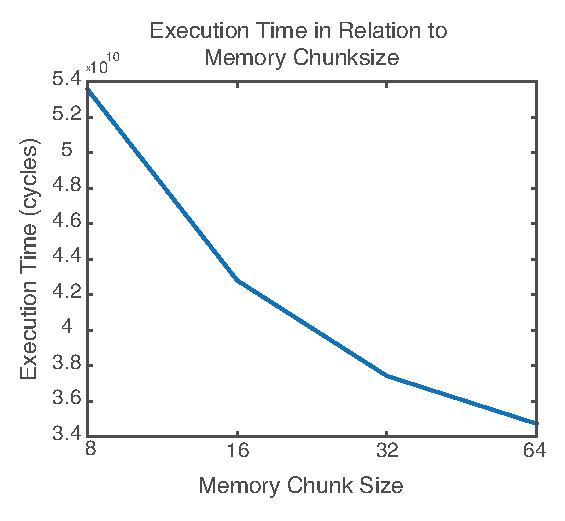
\includegraphics[]{chunkSizes.eps}
\end{center}


\end{document}
